\subsubsection{Design}
\paragraph{Purpose}
The Public Communication Crew is tasked with the essential responsibility of ensuring clear, accurate, and timely information dissemination during emergency situations. This includes relaying updates between emergency teams and the public, maintaining historical records for decision-making, and crafting engaging and informative public communications.

\paragraph{Changes}
Initially, the tasks of the Public Communication Crew (PCC) were planned in a different order and with a distinct execution flow. A comparison of the initial and updated workflows is presented in \textbf{Figure} \ref{fig:exc_flow_pc_comparison}. In the updated process, the first task has been removed, and a new task has been added to consolidate all the information into the desired format. Additionally, the steps involving the Mayor's approval and social media commentary are now performed asynchronously.

\begin{figure}[htbp]
    \centering
    \begin{subfigure}[b]{0.49\textwidth}
        \centering
        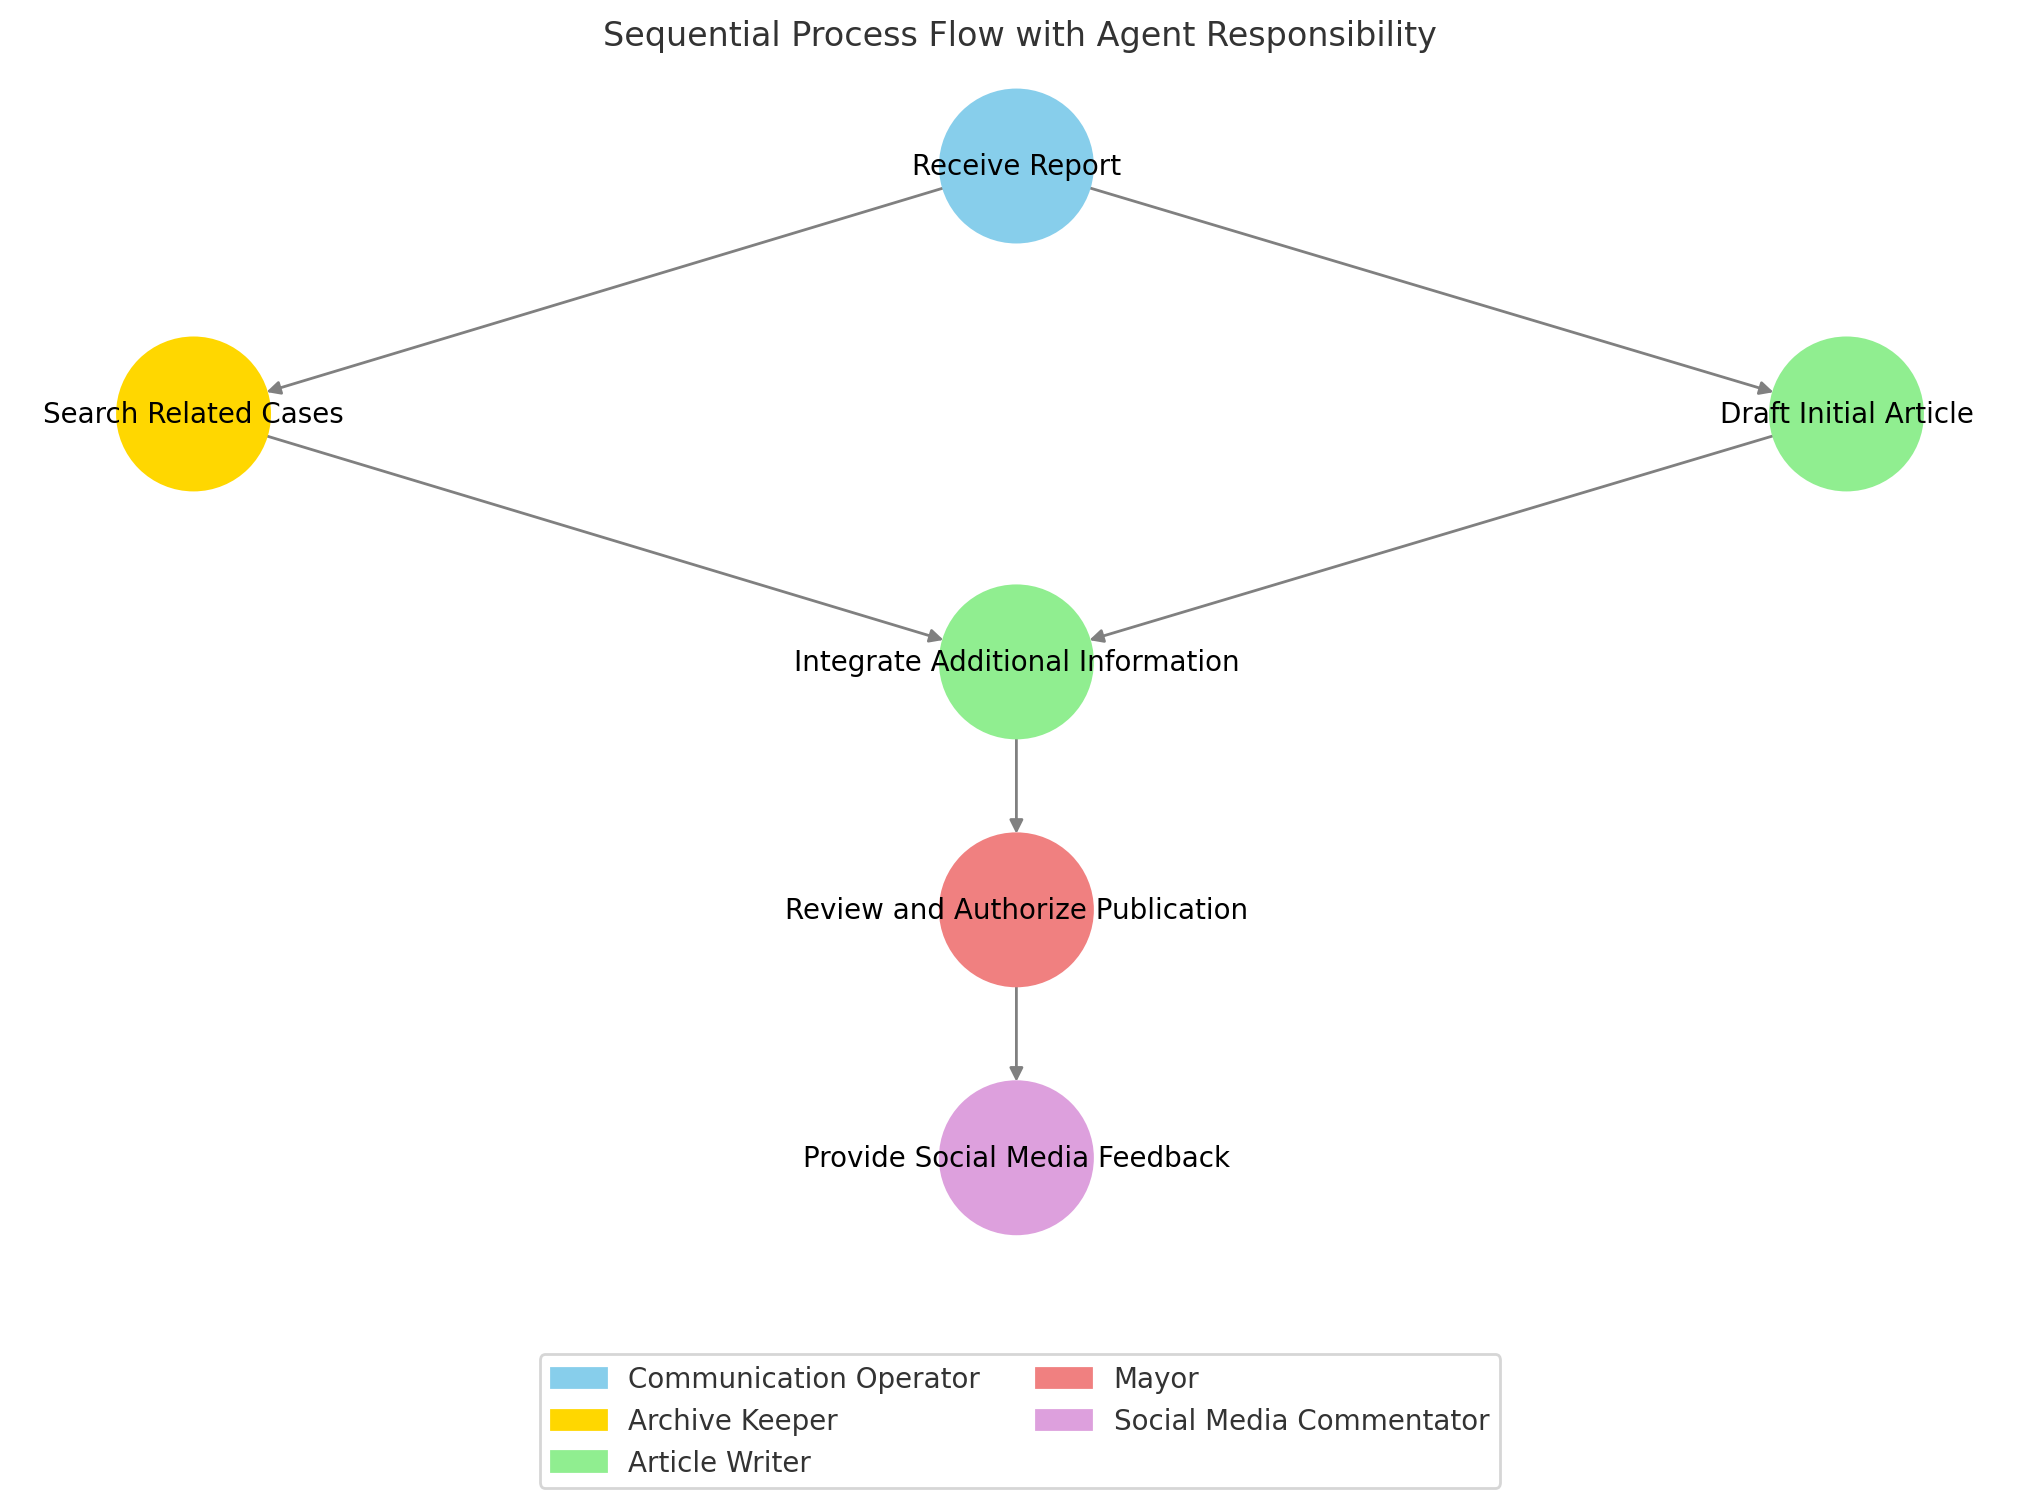
\includegraphics[width=\textwidth]{figures/PC-process.png}
        \caption{Initial process}
        \label{fig:initial_process}
    \end{subfigure}
    \hfill
    \begin{subfigure}[b]{0.49\textwidth}
        \centering
        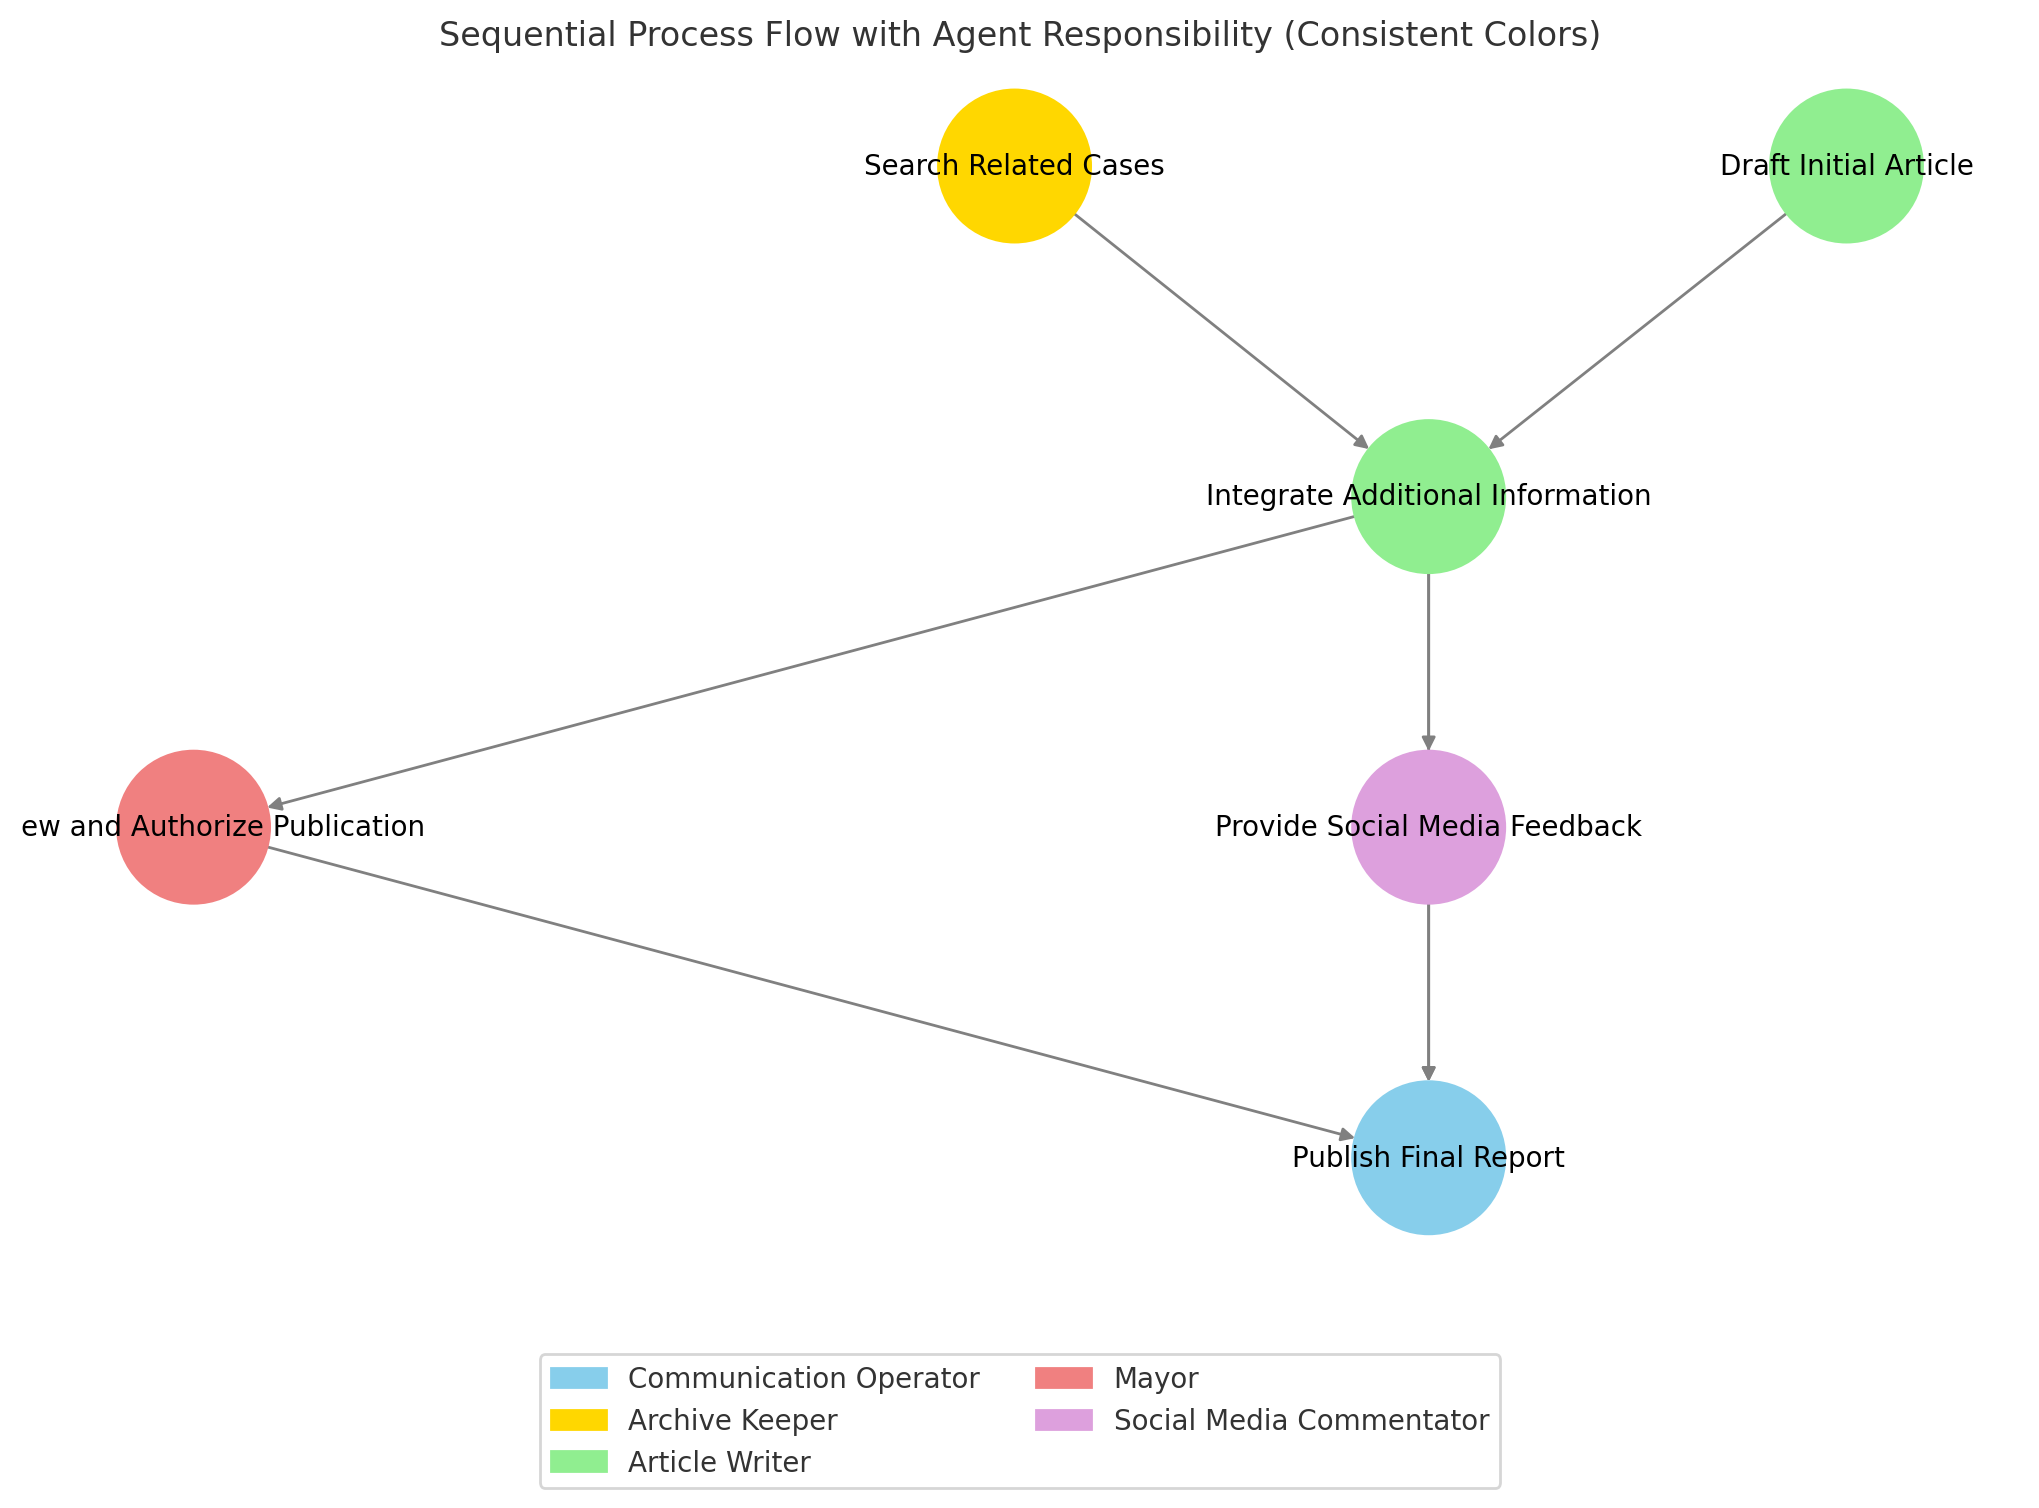
\includegraphics[width=\textwidth]{figures/PC-process-updated.png}
        \caption{Updated process}
        \label{fig:updated_process}
    \end{subfigure}
    \caption{Comparison of the Public Communication Crew's execution flow. (a) shows the initial process, while (b) illustrates the updated process with task removal, task addition, and asynchronous steps.}
    \label{fig:exc_flow_pc_comparison}
\end{figure}

\paragraph{Structure and Components}
The Public Communication Crew leverages the \texttt{CrewBase} framework to orchestrate its agents and tasks, ensuring cohesive and efficient operations. The key components of the design are:

\begin{itemize}
    \item \textbf{Agents:}
    \begin{itemize}
        \item \texttt{communication\_operator}: Relays information between the flow and the public communication team, acting as the primary joint to ensure clarity, correctness and structured format.
        \item \texttt{archive\_keeper}: Manages and retrieves historical data related to past incidents, supporting informed decision-making and comparative analysis.
        \item \texttt{article\_writer}: Drafts and refines articles for public dissemination, focusing on clear and engaging communication.
        \item \texttt{mayor}: Reviews and approves public communications to ensure alignment with city policies and standards.
        \item \texttt{social\_media\_commentator}: Provides lighthearted, constructive feedback on emergency responses, engaging the public while maintaining morale.
    \end{itemize}
    \item \textbf{Tasks:}
    \begin{itemize}
        \item \texttt{search\_related\_cases}: Analyzes historical records to identify similar incidents, highlighting trends and providing context for current events.
        \item \texttt{draft\_initial\_article}: Crafts clear and concise initial drafts of public articles based on structured incident data.
        \item \texttt{integrate\_additional\_information}: Refines drafts by integrating relevant historical or supplementary details, ensuring the article is ready for publication.
        \item \texttt{review\_and\_authorize\_publication}: Evaluates the refined draft for quality and policy alignment, providing final approval or feedback.
        \item \texttt{provide\_social\_media\_feedback}: Offers public-facing commentary that combines wit and constructive critique to enhance communication strategies.
        \item \texttt{publish\_final\_communication}: Consolidates all elements into a cohesive, structured and definitive public communication ready for dissemination.
    \end{itemize}
    \item \textbf{Crew:}
    The crew is constructed using the \texttt{Crew} class, which integrates the agents and tasks into a seamless workflow. This design ensures effective progression from incident analysis and draft creation to final public dissemination and archival.
\end{itemize}
The modular design of the Public Communication Crew enables it to adapt to a wide range of scenarios, ensuring accurate, engaging, and timely communication with both internal teams and the public.
